\let\textcircled=\pgftextcircled



\chapter{Literature Review}
\label{chap:lit_review}

\subsection{Components of a Self Driving Car}

Most self-driving cars consist of 4 main components: 
\begin{itemize}
	\item \textbf{LiDAR} - LiDAR provides highly detailed 3D information about the evnironment around the vehicle and objects in it. LiDAR operates by sending out pulses of lasers and recording the reflections of the pulses from objects. By comparing this with the time taken for the lasers to be reflected(time of flight) and their direction, the distance of these objects can be calculated and mapped in a point cloud. 
	\begin{equation*}
	distance = \frac{time \times \text{speed of light}}{2}
	\end{equation*}
	
	To achieve a high level of accuracy, the LiDAR has to send out a large enough number of lasers in different directions fast enough to create an accurate point cloud representation of the environment around it. As such, LiDAR systems have multiple channels(emitter/receiver pairs) angled vertically that  emit hundreds of thousands of lasers per second.
	
	LiDAR systems require complex optical systems that are expensive to build. As such they are the most expensive sensor in AVs. Consequentially, the cost of production of LiDARs increase greatly as the number of channels increase. More channels allow for more accurate representations of the surrounding environment which is necesary for safer navigation of AVs, however this would not be economically feasible. 
	As such, different companies have are exploring different design methods that are cheap but accurate. 
	Types of LiDAR
	\begin{itemize}
		\item \textbf{Mechanical Mirror}
		\item \textbf{Solid State}
		\item \textbf{Optical Phase Array}
		\item \textbf{Microelectromechanical systems (MEMS)}
		\item \textbf{3D Flash}
	\end{itemize}
	
	
	\item \textbf{Cameras} - Cameras mounted on the vehicle are used for classification and identification of various objects on the road. This is important for recognising traffic rules from traffic signs or road markings as well as determining the nature of objects on the road. 
	Cameras can also be used to create 3D maps of the surrounding environment.By combining two cameras, a stereo image can be captured that provides depth information. Alternatively, by combining a camera and IR Laser sensor for depth estimation, RGB-D images are obtained and mapped in a point cloud.
	
	\item \textbf{Position Estimators} - Position estimators are a group of sensors used for navigation of the vehicle. These include GPS systems, odometers and gryometers. 
	\item \textbf{Distance Sensors} - Distance sensors such as radars and sonars are important for gauging the distance of objects on the road. 
	Radars are the most commonly used distance sensors and they work by transmitting radio waves and recording the reflected radio waves from objects. As compared to cameras and LiDARs, radars work well in a variety of low visibility scenarios such as poor weather. 
	However, the reflectivity of these radio waves depends on the nature of objects, their size, absorbtion characteristics and the transmitting power. As such, it is may not be effective for detecting objects with low absorbtion characteristics such as pedestrians and animals.
	
	\item \textbf{Processing Unit} - In order to process all the data from the sensors in the vehicle, AVs require powerful processing units in order to be able to process all this data in real time. Most of the ML/AI algorithms used for detecting and identifying objects from LiDAR and camera data demand large amounts of processing power. This is achieved through the use of CPUs, GPUs, FPGA or combinations with each other. 

\end{itemize}


\begin{figure}[t]
	\centering
	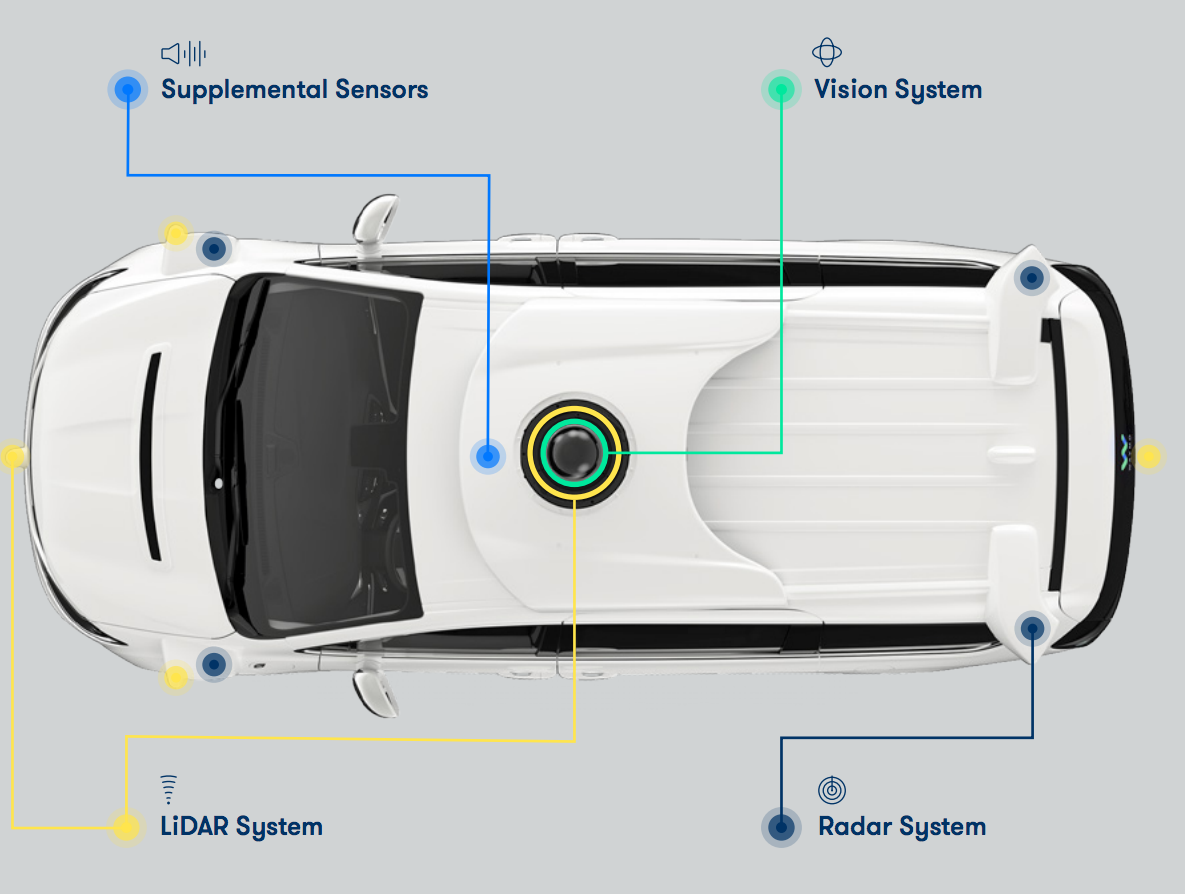
\includegraphics[width=\textwidth]{media/waymo.png}
	\caption{Components of Waymo's Self Driving Car (Waymo)}
	\label{fig:my_label}
\end{figure}

As seen from the table above, a wide range of sensors are used in AVs with each . This is essential for accurate navigation of the AV and therefore multiple sensors are fused together in order to provide enough data to achieve this. Given the large number of sensors, a major inhibiting factor in the production of AVs is the cost of sensors.



\subsection{Legal, Ethical and Economic Considerations}

The classic ethical dilemma for self driving cars poses a scenario whereby AVs are presented with a situation whereby a fatal accident is inevitable. For example, the AV either has to crash into a group of people in order to save the life of a passenger or to crash itself and sacrifice the life of the passenger. This dilemma highlights important legal, ethical and economic considerations to be considered by companies involved in the production of AVs and their corresponding systems. 




According to \cite{gasser2016fundamental}, there are no public laws that cover the  use of independent autonomous vehicles in public spaces. In his article, he cites the fundamental issue as "understanding and accepting the effect of AVs as an independent action by a machine". Due to the lack of public laws on their use, he proposes extending fundamental rights such as the right to life into the framework for creating laws that cover emerging technologies that have an effect on the public, that are otherwise not accounted for in traditional laws. 

Bearing this in mind, it is important to note that despite improvements in traffic safety over the years, 94\% are still caused by human beings with a large majority of them being fatal with the current human error rate being 1 in 100 million miles. This creates a realistic baseline that can then be extended in evaluating the performance of AV systems. As such, if the risk of automation is lesser than the risk of human vehicle control then the AV would be beneficial. Consequently, the AVs are not to be considered as perfect systems.

With regard to economic considerations, car manufucturers involved in the production of AVs have to ensure that their AVs are able to handle numerous scenarios even if they are rare or considered statistically impossible. They should also be required to take legal liability in case any of their system components are defective and result in failures or accidents. This is important for customer trust without which they will not be able to convince customers to buy AVs. In addition, for the adoption of AVs to be widespread, they have to be reasonably priced. With the current prices of the the various components, the adoption of AVs at the moment is not viable. 


\section{Object Detection}

AVs have three main modes of operation namely,
\begin{itemize}
	\item \textbf{Perception} - This is the first step which involves processing the input from the sensors. In this mode tasks such as object detection and tracking, lane detection, traffic sign detection and recognition are performed.
	\item \textbf{Planning} - After the detection and recognition tasks are performed in the perception stage, route and trajectory planning algorithms are performed. These algorithms are required to handle complex situations to ensure safety of the passengers and other road users. 
	\item \textbf{Control} - This stage involves the execution of the plans created in the previous stage. This stage is crucial as the actuators involved in steering and movement have to be able to be able to accurately follow the plans. This involves calculation of energy and forces. At this stage the trajectories and movement of other road users and objects have to be calculated in order to anticipate and avoid any accidents. 
	
\end{itemize}

A recurring theme that is central to the operation of AVs is object detection. Object detection is crucial for safe operation of AVs as it forms the first step before any planning and control. As such, various companies have been working to come up with accurate object detection systems through different combination of sensors in order to achieve this. To achieve real-time results, deep learning techniques are being developed for this task. 


Following the discussion in the previous section, a few requirements have to be fulfilled for mainstream AV adoption. 
These requirements are as below:
\begin{itemize}
    \item \textbf{Robust}
    \item \textbf{Reproducible}
    \item \textbf{Validatable}
    \item \textbf{Viable}
\end{itemize}











\section{Conclusion}




